\section{Basic CNN Seq2seq Model}
\label{sec:model}

We first describe a multi-layer convolutional sequence-to-sequence model~\footnote{\url{https://github.com/facebookresearch/fairseq-py}.} \cite{gehring2017convs2s,CunBDHHHJ89}
with an attention mechanism, which is the basic model which we will extend to support
length constraints. \figref{fig:cnn} illustrates the model.

\begin{figure}[th!]
\centering
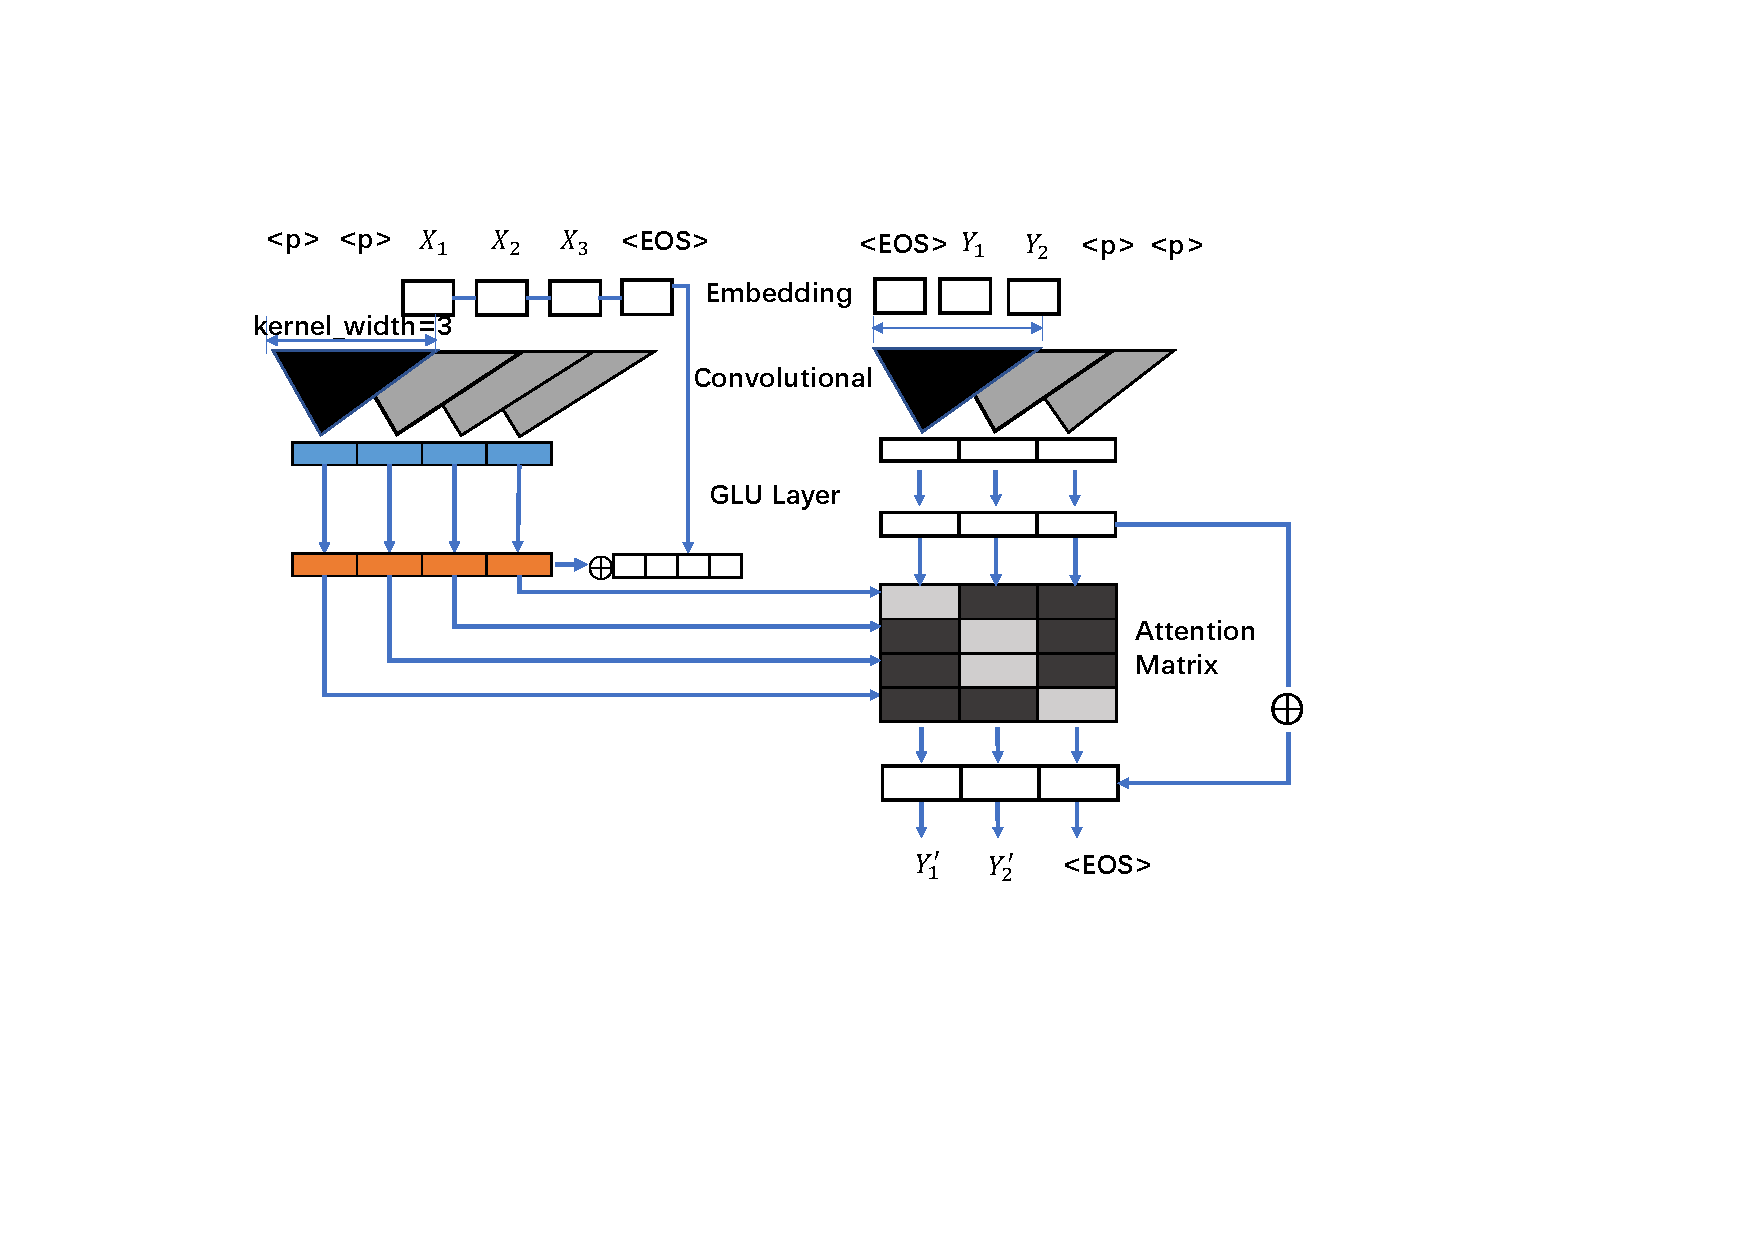
\includegraphics[width=1.0\columnwidth]{figure/cmodel}
\caption{CNN sequence-to-sequence model} \label{fig:cnn}
\end{figure}

Given a sequence of tokens $\textbf{x} = (x_{1},x_{2},...,x_{m})$ in the
source document and a sequence of tokens
$\textbf{y} = (y_{1}, y_{2},..., y_{n})$ in the target summary (i.e. $m>n$),
the goal of summarization is to estimate the conditional probability
$p(\textbf{y}|\textbf{x})$:
\begin{equation}
p(\textbf{y} | \textbf{x}) \!=\! {\prod^T_{t} {p(y_{t} | y_{1}, y_{2},..., y_{t-1}, \textbf{x}})}
\end{equation}

After combining word vectors with their absolute positions in the document,
we obtain the input sequence
$\textbf{X}=(X_{1},...,{Xm})$ and output sequence $\textbf{Y}=(Y_{i},...,Y_{n})$
to the seq2seq model.
%These sequences contain semantic and positional information. In this model,
%encoder and decoder are both based on multi-layers convolutional
%networks~\citep{CunBDHHHJ89}.
We use $\textbf{z}=(z^l_{1}, z^l_{2},..., z^l_{m})$ and
$\textbf{h}=(h^l_{1}, h^l_{2},..., h^l_{n})$
to denote the output of the encoder and decoder in $l$-th layer.
Each element of the output sequence generated by the decoder network
is fed back into the next layer of decoder network.
Next, we use a GLU \cite{DauphinFAG17} and residual connections to get
output of convolutional part in each layer \cite{HeZRS16}:
%GLU is non-linearity and is used as a gate. This process is described
%as follows.
\begin{equation}
h^l_{i} \!=\! GLU(W^l[h^{l-1}_{i-k/2},...,h^{l-1}_{i+k/2}]\!+\!b^l)\!+\!h^{l-1}_{i}
\end{equation}

We compute the probability distribution of generating the
next elements $y_{i+1}$ based
on the current state and transform the top decoder output $h^L_{i}$ via softmax:
\begin{equation}
p(y_{i+1}|y_{1},...,y_{i},\textbf{x})\!=\!softmax(W_{o}h^L_{i}\!+\!b_{o})
\end{equation}

In addition, a multi-step attention mechanism that connects the encoder and
decoder is used in each decoder layer:
%It connects the encoder and decoder model after each GLU.
%To compute the attention, we define the decoder
%state $d^l_{i}$ for attention as following:
\begin{equation}
d^l_{i}\!=\!W^l_{d}h^l_{i}\!+\!b^l_{d}+Y_{i}
\end{equation}

The attention $c^l_{i}$ is a weighted sum of the encoder outputs.
The weights $a^l_{ij}$ are based on the decoder states.
%It can provide the distribution of next token given the input sequence.
\begin{align}
a^l_{ij} \!&=\! \frac {\exp(d^l_{i}\cdot z^u_{j})}{\sum^m_{t=1} \exp(d^l_{i}\cdot z^u_{t})} \\
c^l_{i}  \!&=\! \sum^m_{j=1} a^l_{ij}(z^u_{j}+X_{j})
\end{align}

At last, we add $c^l_{i}$ to the current decoder elements $h^l_{i}$,
which forms the final output or the
input of the next layer in the decoder.

%The advantage of the multi-layer convolutional neural networks is that
%it forms a hierarchical structure over the input sequence.
%The lower layers captures the correlations between nearby tokens in
%the sequence, while the higher layers encodes the longer range
%correlations within the sequence. Exactly what information is important
%during the information propagation between the layers is determined
%by GLU.

